\documentclass[conference]{IEEEtran}
\IEEEoverridecommandlockouts

\usepackage{iftex}
\ifPDFTeX
  \usepackage[utf8]{inputenc}
  \usepackage[T1]{fontenc}
\else
  \usepackage{fontspec}
\fi

\usepackage[spanish,es-noindentfirst]{babel}
\usepackage{graphicx}
\usepackage{amsmath,amssymb}
\usepackage{booktabs}
\usepackage{array}
\usepackage{url}
\usepackage[hidelinks]{hyperref}

\graphicspath{{figures/}}

\begin{document}

\title{Clasificación de Señales Eco-Acústicas para la\\
Identificación Autónoma de Especies Faunísticas}

\author{
\IEEEauthorblockN{Integrante 1}
\IEEEauthorblockA{Universidad de Ingeniería y Tecnología\\
Lima, Perú\\
integrante1@utec.edu.pe}
\and
\IEEEauthorblockN{Integrante 2}
\IEEEauthorblockA{Universidad de Ingeniería y Tecnología\\
Lima, Perú\\
integrante2@utec.edu.pe}
\and
\IEEEauthorblockN{Integrante 3}
\IEEEauthorblockA{Universidad de Ingeniería y Tecnología\\
Lima, Perú\\
integrante3@utec.edu.pe}
}

\maketitle

\begin{abstract}
Se aborda la clasificación automatizada de señales eco-acústicas para la
identificación autónoma de cinco especies faunísticas a partir de descriptores
tabulares MFCC ($X \in \mathbb{R}^{64}$). Se desarrolló un pipeline integral que
contrasta la reducción de dimensionalidad lineal (PCA) frente a métodos de
variedades múltiples (UMAP, t-SNE), explora la estructura no supervisada mediante
modelos de mezcla gaussiana (GMM) y densidad (DBSCAN), y compara un perceptrón
multicapa (MLP) contra modelos de ensamble por gradiente (XGBoost, LightGBM). El
análisis evidenció un fuerte solapamiento inter-especie: las técnicas no
supervisadas no recuperan la etiqueta biológica (ARI $\approx 0$), lo que motiva el
enfoque supervisado. LightGBM obtuvo el mejor desempeño (F1-macro $=0{.}441$) con un
costo de inferencia 30--40 veces menor que el MLP. Finalmente, se demostró que el
umbral de confianza prescrito del 85\,\% resulta inalcanzable bajo el solapamiento
observado, por lo que se propone recalibrar las políticas de moderación a partir de
la curva exactitud--cobertura.
\end{abstract}

\begin{IEEEkeywords}
clasificación eco-acústica, MFCC, reducción de dimensionalidad, clustering,
perceptrón multicapa, gradient boosting, clasificación selectiva.
\end{IEEEkeywords}

\section{Resumen Ejecutivo e Introducción al Espacio Vectorial}

El monitoreo acústico pasivo permite censar biodiversidad en regiones extensas sin
intervención humana, pero genera volúmenes de audio cuya anotación manual es
inviable. El presente trabajo aborda la clasificación automatizada de especies a
partir de un conjunto tabular preprocesado de 1906 observaciones de entrenamiento y
477 de prueba. Cada registro queda descrito por un vector de características
$X \in \mathbb{R}^{64}$ correspondiente a coeficientes cepstrales en escala de Mel
(MFCC, \texttt{mel\_0}--\texttt{mel\_63}), que condensan las propiedades de frecuencia
y timbre de la señal. La variable objetivo \texttt{species\_id} codifica cinco
especies ---dos anfibios (\emph{Leptodactylus discodactylus}, \emph{Osteocephalus
taurinus}) y tres aves (\emph{Chiroxiphia lineata}, \emph{Saltator grossus},
\emph{Pheucticus chrysopeplus})--- distribuidas de forma asimétrica (razón de
desbalance máximo/mínimo $=2{.}0$). La arquitectura completa de la solución, desde la
ingesta del CSV hasta la moderación por umbrales, se ilustra en la
Fig.~\ref{fig:arch}.

Dos particularidades del conjunto condicionan el diseño metodológico. Primero, el
indicador binario \texttt{is\_tp} (\emph{true positive}) revela que solo el
13{.}2\,\% de los registros se encuentra verificado; el resto constituye señal de
fiabilidad incierta asimilable a ruido ambiental. Segundo, las 1906 filas provienen
de únicamente 1597 grabaciones (\texttt{recording\_id}), con hasta cinco ventanas por
grabación, y 122 grabaciones aparecen simultáneamente en los conjuntos de
entrenamiento y prueba. Dicha superposición implica fuga de información en la
partición provista, por lo que toda validación interna se realizó con particiones
agrupadas por \texttt{recording\_id}. El código fuente y las instrucciones de
reproducción se encuentran en el repositorio público
\url{https://github.com/USUARIO/p2-eco-acoustic}.

\begin{figure*}[!t]
\centering
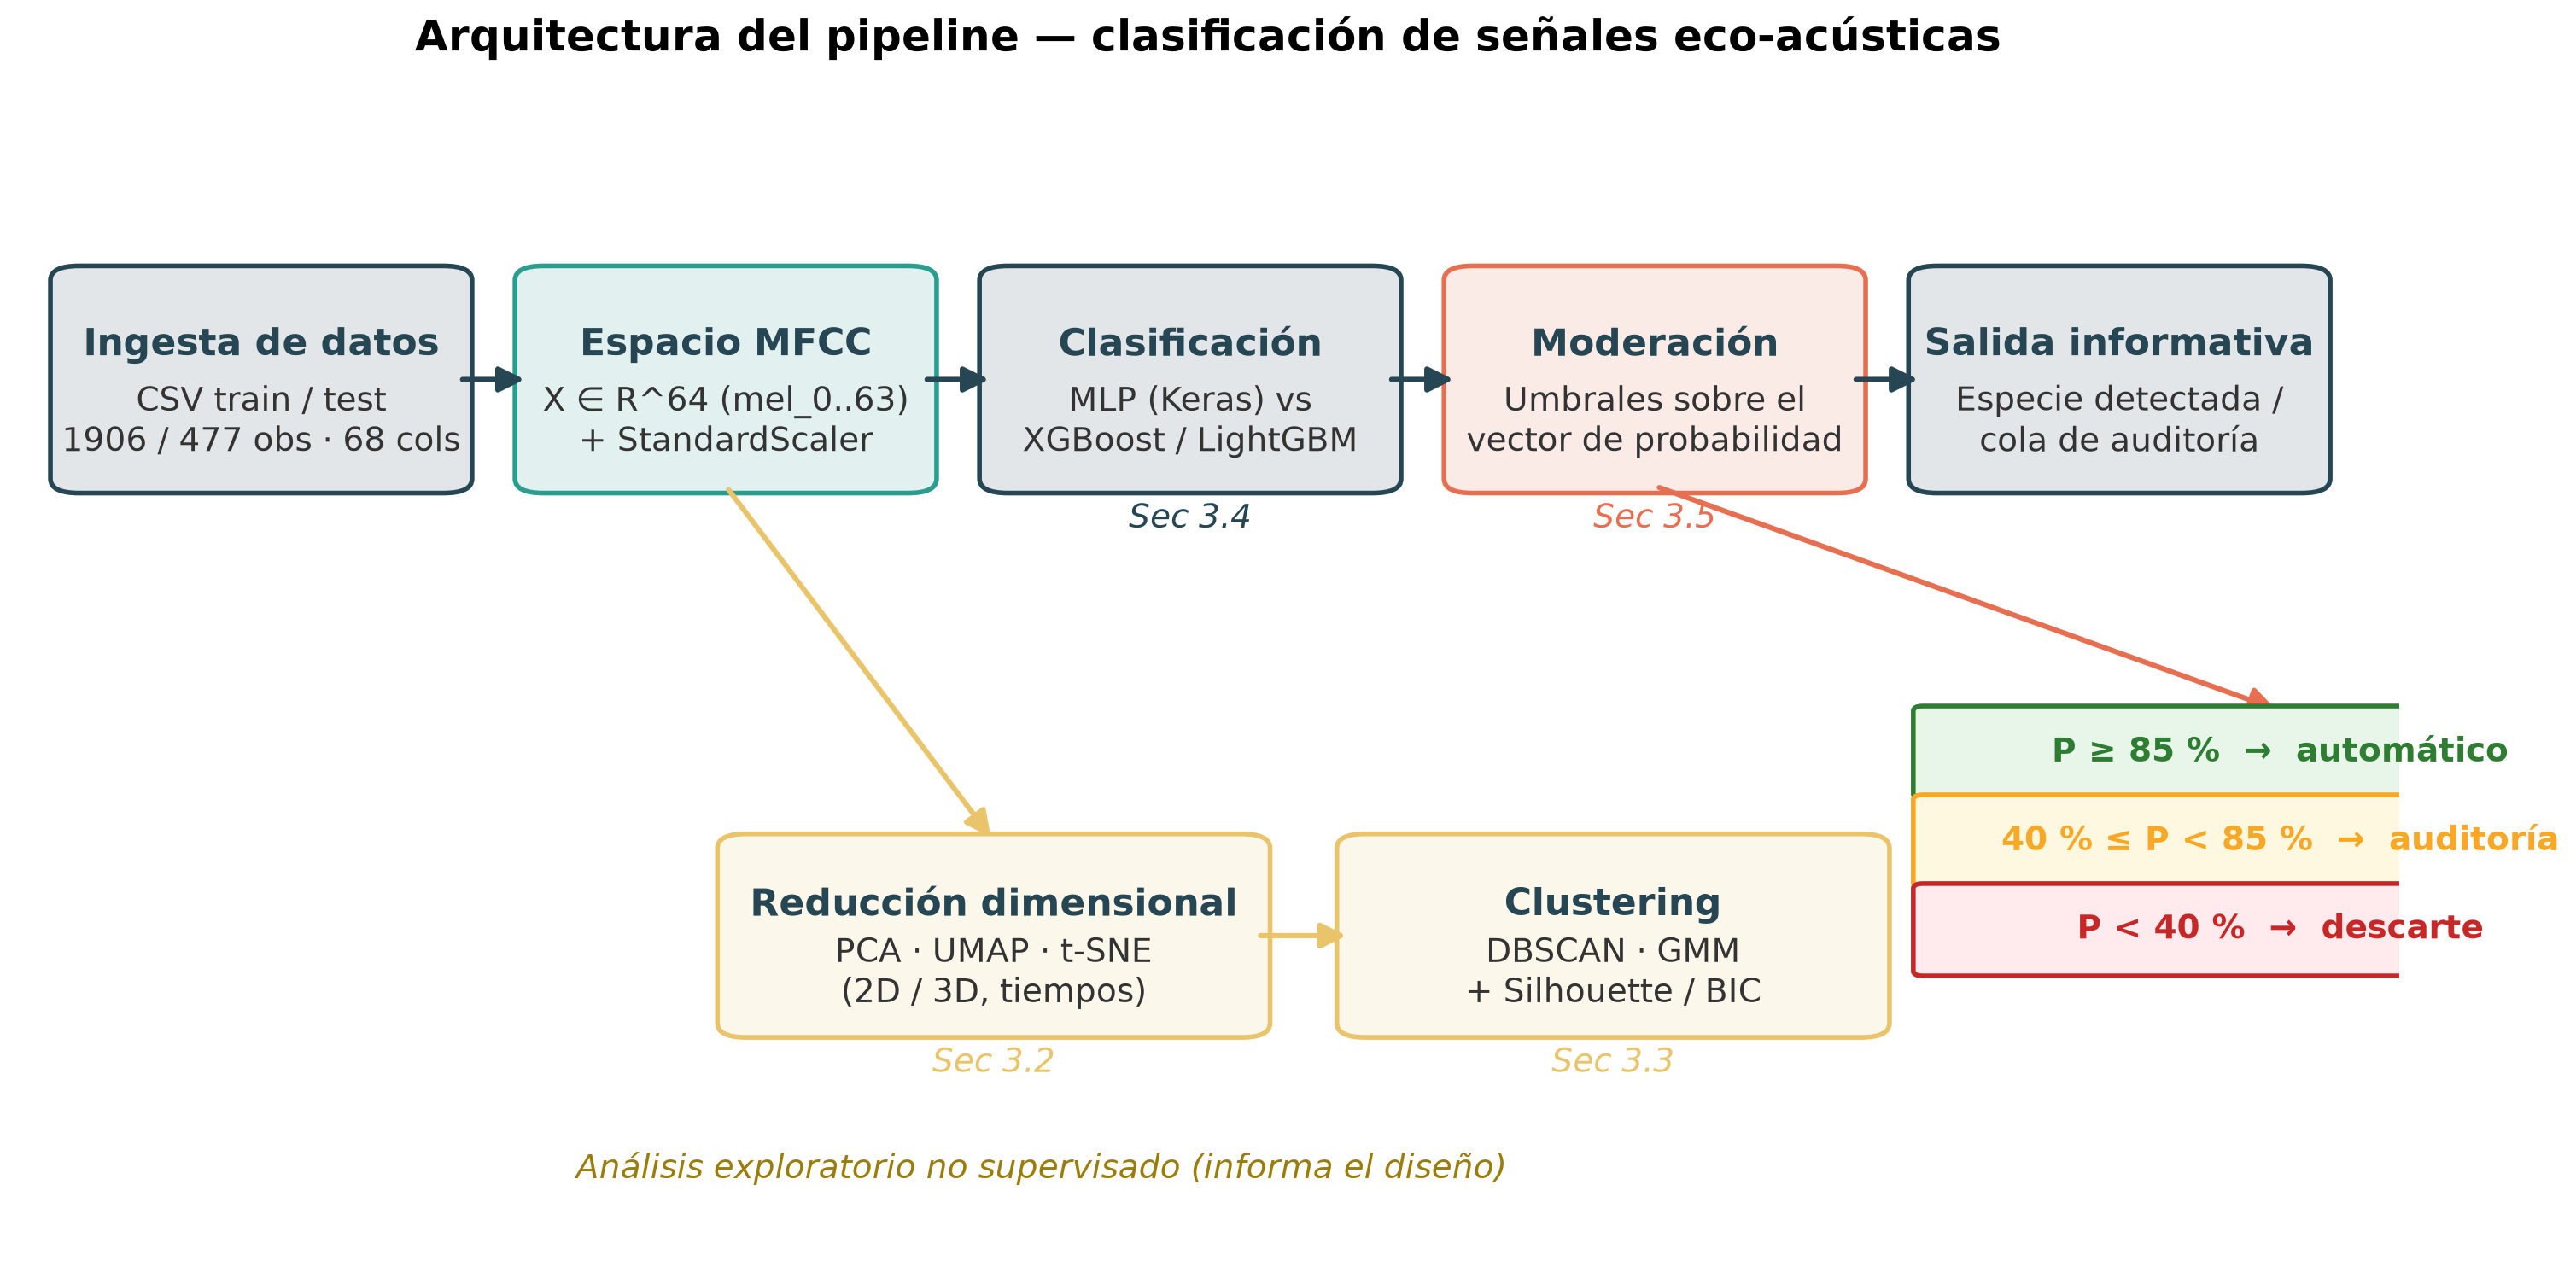
\includegraphics[width=\textwidth]{architecture.png}
\caption{Arquitectura del pipeline. El flujo de inferencia (fila superior) conecta la
ingesta del CSV con el espacio MFCC, la clasificación supervisada y la moderación por
umbrales; la rama inferior corresponde al análisis exploratorio no supervisado que
informa las decisiones de diseño.}
\label{fig:arch}
\end{figure*}

\section{Exploración Geométrica y Reducción de Dimensionalidad}

Se contrastó un método lineal (PCA) frente a dos técnicas de variedades múltiples
(t-SNE~\cite{tsne} y UMAP~\cite{umap}), proyectando el espacio MFCC estandarizado a dos y tres dimensiones
(Fig.~\ref{fig:dimred2d}). El análisis de varianza reveló que PCA requiere siete
componentes para retener el 90\,\% de la varianza y once para el 95\,\%; en dos
dimensiones retiene apenas el 67{.}1\,\% y en tres el 76{.}7\,\%
(Fig.~\ref{fig:scree}). La preservación de la estructura local se cuantificó mediante
el índice de \emph{trustworthiness} y la separabilidad de clases vía $k$NN con
validación cruzada estratificada en el espacio proyectado, según se resume en la
Tabla~\ref{tab:dimred}.

\begin{table}[!t]
\caption{Comparación de los métodos de reducción de dimensionalidad.}
\label{tab:dimred}
\centering
\begin{tabular}{llcccc}
\toprule
Método & Dim & Tiempo (s) & Var. ret. & Trust. & $k$NN acc. \\
\midrule
PCA   & 2 & 0.002 & 0.671 & 0.867 & 0.311 \\
PCA   & 3 & 0.002 & 0.767 & 0.940 & 0.327 \\
t-SNE & 2 & 9.11  & ---   & 0.987 & 0.369 \\
t-SNE & 3 & 12.00 & ---   & 0.992 & 0.388 \\
UMAP  & 2 & 15.78 & ---   & 0.976 & 0.374 \\
UMAP  & 3 & 5.90  & ---   & 0.986 & 0.372 \\
\bottomrule
\end{tabular}
\end{table}

\begin{figure*}[!t]
\centering
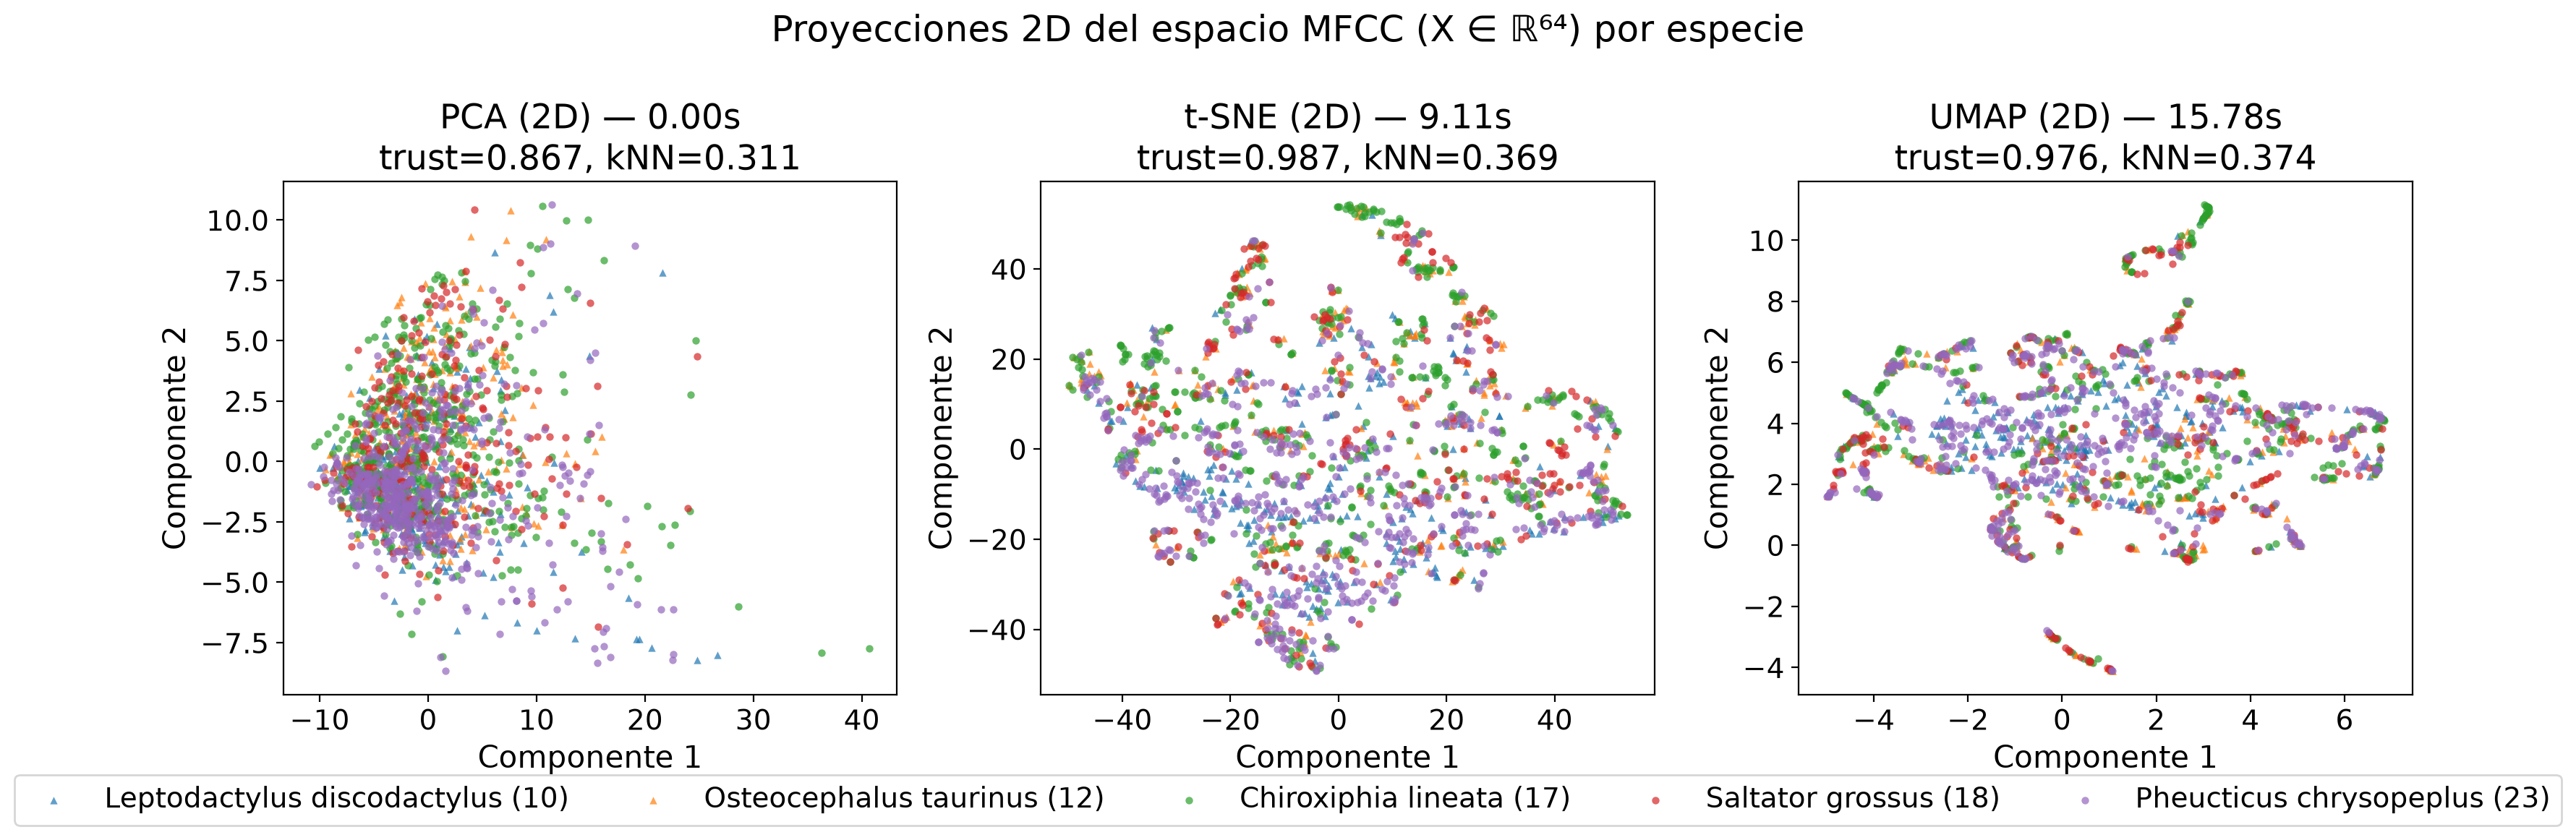
\includegraphics[width=\textwidth]{dimred_2d_panels.png}
\caption{Proyecciones 2D del espacio MFCC por especie. PCA preserva la varianza
global pero distorsiona los vecindarios; t-SNE y UMAP recuperan estructura local a
mayor costo. Las clases permanecen fuertemente solapadas en todos los casos.}
\label{fig:dimred2d}
\end{figure*}

\begin{figure}[!t]
\centering
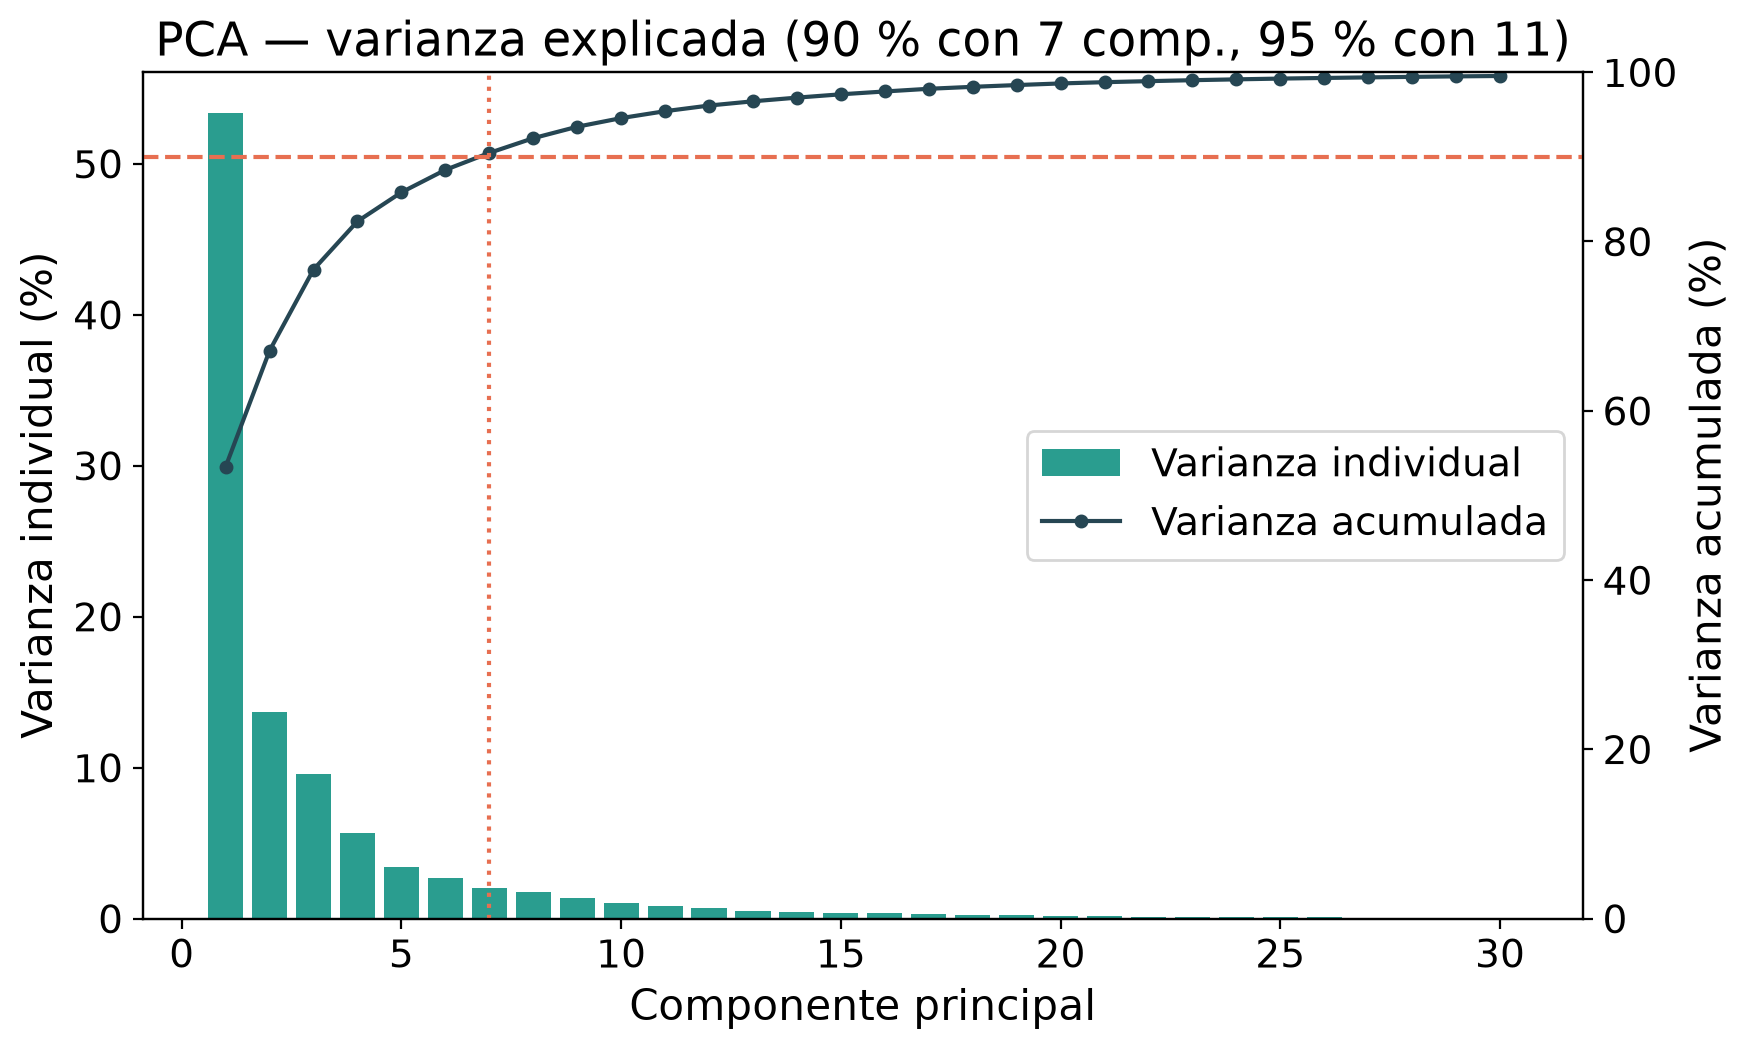
\includegraphics[width=\columnwidth]{dimred_pca_scree.png}
\caption{Varianza explicada individual y acumulada de PCA. Se requieren siete
componentes para alcanzar el 90\,\% de la varianza.}
\label{fig:scree}
\end{figure}

Se concluye que PCA, aun siendo prácticamente instantáneo (0{.}002~s) y ofreciendo
una base interpretable por varianza, distorsiona los vecindarios locales
(\emph{trustworthiness} de 0{.}867 en 2D). Las técnicas no lineales elevan dicho
índice a $\sim$0{.}98--0{.}99 a un costo de 6--16~s, sin preservar interpretabilidad
por varianza. Resulta crítico que la separabilidad $k$NN no supera 0{.}39 en ningún
espacio, apenas por encima del baseline de clase mayoritaria ($\sim$0{.}29): las
cinco especies se solapan intensamente en el dominio MFCC, lo que anticipa la
dificultad de la tarea supervisada. Adicionalmente, los registros verificados
(\texttt{is\_tp}$=1$) aparecen dispersos sin formar región propia, confirmando que
\texttt{is\_tp} es una bandera de calidad de etiqueta y no una clase geométricamente
separable.

\section{Minería de Patrones y Estructuras de Clustering}

Se implementaron dos paradigmas distintos sobre el espacio PCA que retiene el 90\,\%
de la varianza (7D): un modelo probabilístico (\emph{Gaussian Mixture Model}, GMM) y
uno basado en densidad (DBSCAN). Para el GMM se barrió $k \in [2,10]$ evaluando BIC,
AIC, Silhouette~\cite{silhouette}, Davies--Bouldin y Calinski--Harabasz; para DBSCAN se seleccionó
$\varepsilon$ mediante el codo del grafo de $k$-distancias y un barrido que reporta
número de clústeres, fracción de ruido y Silhouette.

Las métricas internas resultaron contradictorias: BIC y AIC decrecen monótonamente
---favoreciendo el máximo $k=10$, síntoma típico de ausencia de componentes
gaussianas separadas--- mientras que Silhouette (máximo en $k=2$) y
Calinski--Harabasz (máximo en $k=3$) favorecen particiones gruesas. No se identificó
un número de grupos con clústeres compactos y bien separados. El contraste externo
con las etiquetas reales (Fig.~\ref{fig:clusters}) fue concluyente: ninguna partición
recupera las especies (ARI $\approx 0{.}0$--$0{.}05$, NMI $\approx 0$), ni se alinea
con el tipo de fauna (anfibio/ave) ni con el \texttt{songtype} (ARI $\approx 0$). Se
infiere que la estructura geométrica dominante del espacio MFCC obedece a variación
acústica de fondo a nivel de grabación, y no a la etiqueta biológica. Este hallazgo
justifica el recurso al aprendizaje supervisado de la Sección~\ref{sec:clf} para
aislar las direcciones discriminantes que los métodos no supervisados no exponen.

\begin{figure*}[!t]
\centering
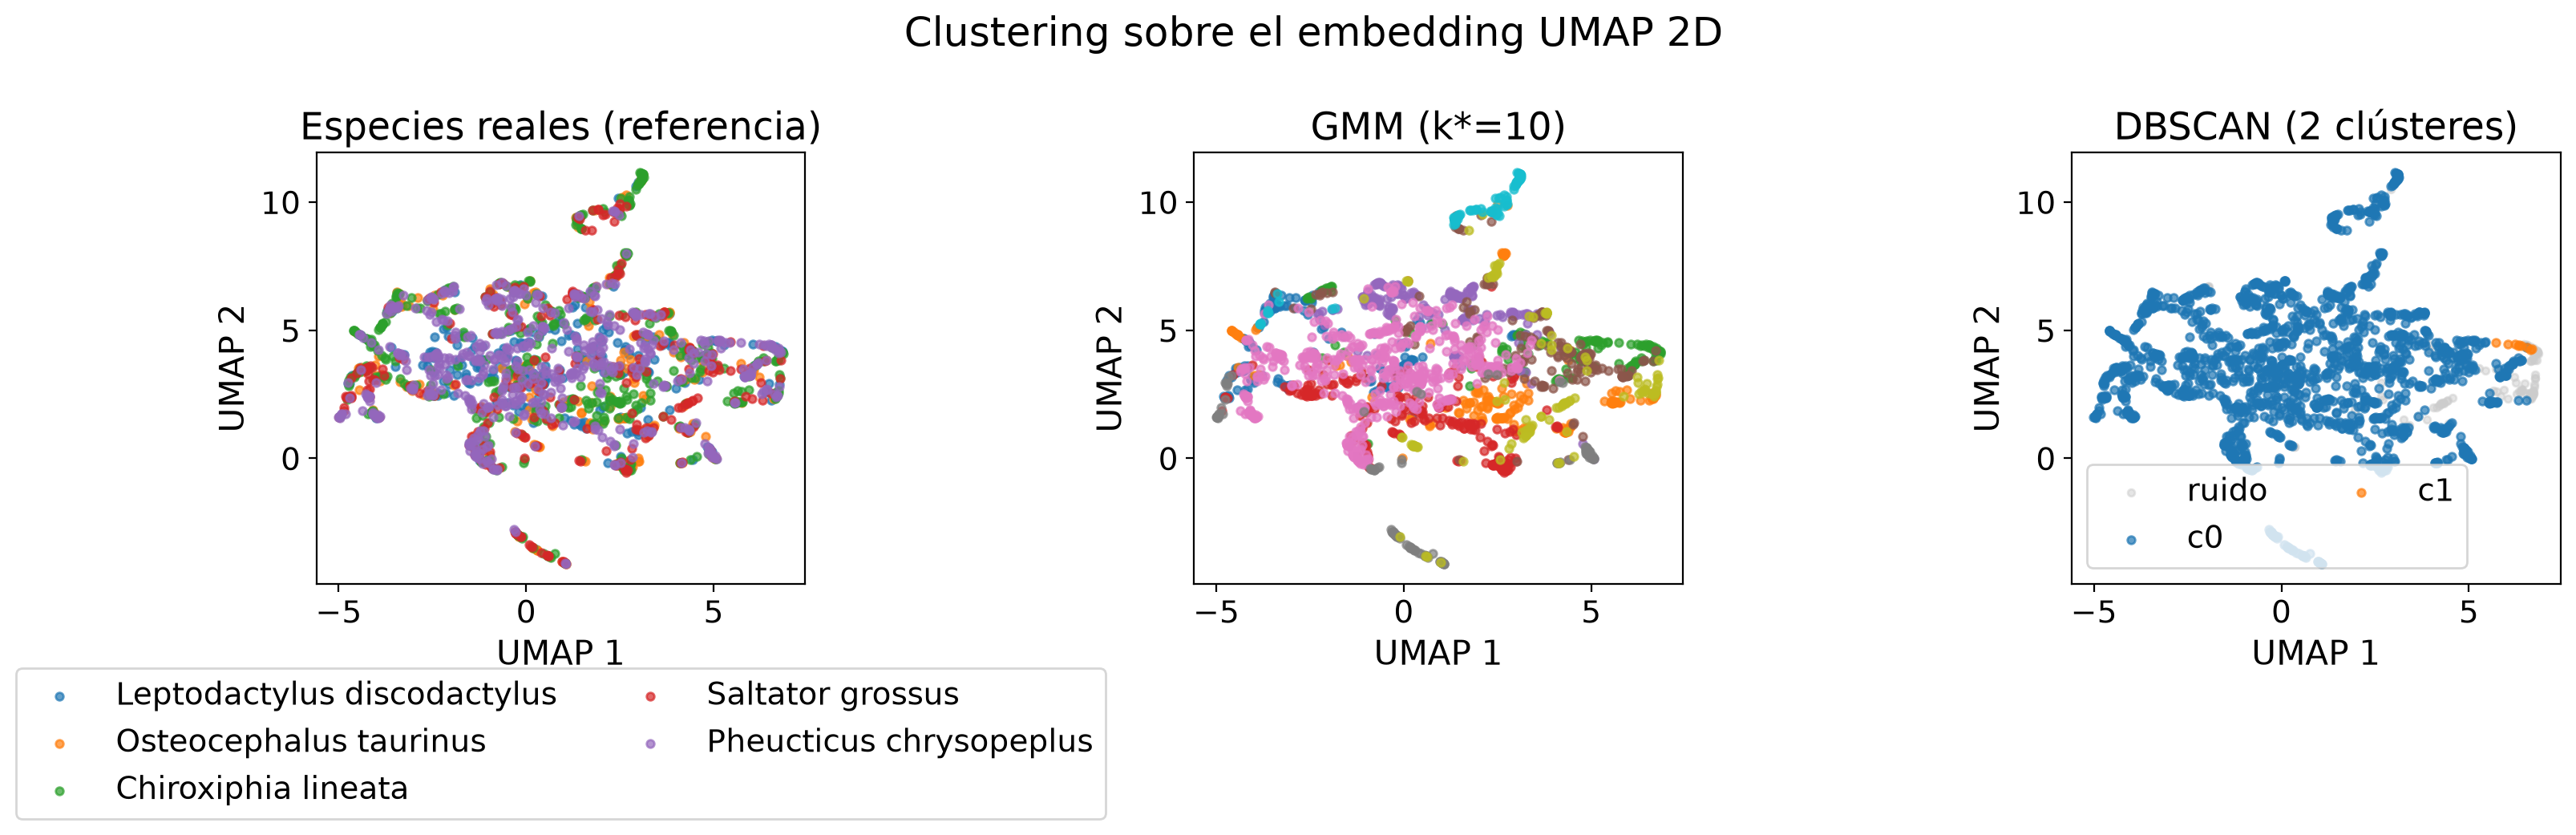
\includegraphics[width=\textwidth]{clustering_umap_compare.png}
\caption{Clustering sobre el embedding UMAP 2D. Ni el GMM ni DBSCAN reproducen la
distribución de especies reales (panel izquierdo); las particiones obtenidas no se
corresponden con ninguna etiqueta disponible.}
\label{fig:clusters}
\end{figure*}

\section{Arquitectura de Clasificación: MLP vs. Modelos de Ensamble}
\label{sec:clf}

\textbf{Función de pérdida.} Para la clasificación multiclase se empleó la entropía
cruzada categórica, definida sobre $N$ muestras y $C=5$ clases como
\begin{equation}
\mathcal{L} = -\frac{1}{N}\sum_{i=1}^{N}\sum_{c=1}^{C} y_{ic}\,\log(p_{ic}),
\end{equation}
donde $p_{ic} = \mathrm{softmax}(z_i)_c$ es la probabilidad predicha y $y_{ic}$ la
codificación \emph{one-hot} de la clase verdadera. El desbalance se compensó con
ponderación de clases inversamente proporcional a su frecuencia. La topología del MLP
final se detalla en la Tabla~\ref{tab:topo}.

\begin{table}[!t]
\caption{Topología del MLP final (entropía cruzada categórica, optimizador Adam,
$\eta=10^{-3}$, \emph{early stopping}).}
\label{tab:topo}
\centering
\begin{tabular}{lccc}
\toprule
Capa & Unidades & Activación & Parámetros \\
\midrule
Entrada        & 64  & ---     & 0 \\
Densa 1        & 128 & ReLU    & 8\,320 \\
Dropout (0.3)  & --- & ---     & 0 \\
Densa 2        & 64  & ReLU    & 8\,256 \\
Dropout (0.3)  & --- & ---     & 0 \\
Salida         & 5   & softmax & 325 \\
\midrule
\multicolumn{3}{l}{Total entrenable} & 16\,901 \\
\bottomrule
\end{tabular}
\end{table}

\textbf{Estrategia de regularización.} Se estudió el efecto de la posición relativa
de las capas de Dropout~\cite{dropout} y Batch Normalization~\cite{batchnorm} sobre la estabilidad de las curvas de
aprendizaje (Fig.~\ref{fig:curves}), comparando cinco configuraciones del bloque
oculto. El análisis evidenció que el factor determinante de la estabilidad es la
\emph{presencia de Dropout}, no su orden relativo: las tres variantes con Dropout
mantienen la pérdida de validación plana ($\sim$1{.}35) durante 100 épocas, mientras
que las configuraciones \emph{BN sin Dropout} y \emph{sin regularización}
sobreajustan ---la pérdida de entrenamiento decae pero la de validación diverge---.
Entre las variantes con Dropout, el orden BN$\rightarrow$Dropout frente a
Dropout$\rightarrow$BN apenas altera el F1-macro. La arquitectura final se seleccionó
por mínima pérdida de validación en convergencia, criterio que descarta las variantes
sobreajustadas.

\begin{figure*}[!t]
\centering
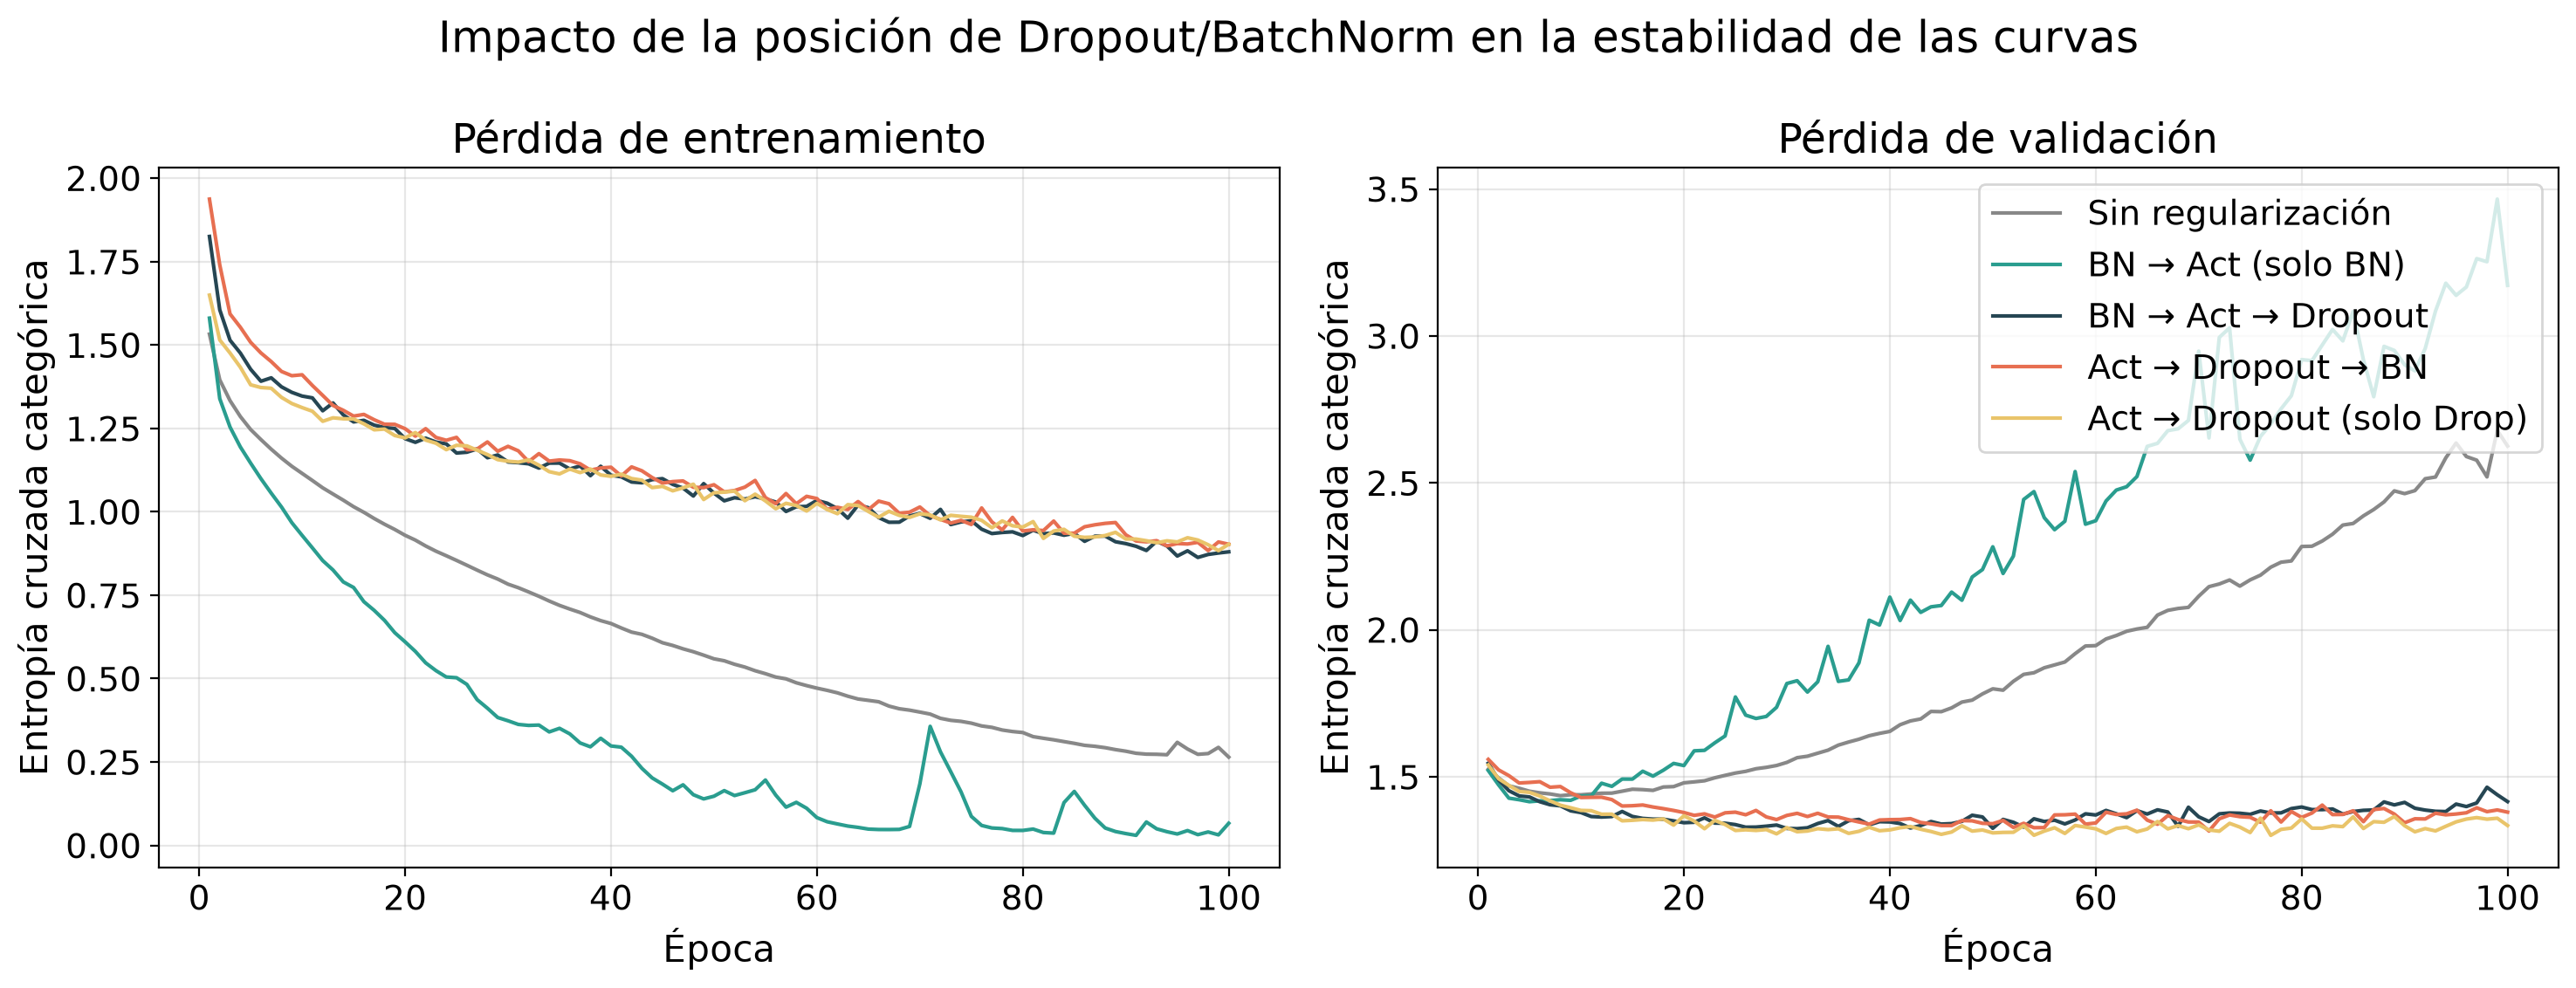
\includegraphics[width=\textwidth]{clf_learning_curves.png}
\caption{Impacto de la posición de Dropout/BatchNorm en la estabilidad. La presencia
de Dropout (no su orden) mantiene plana la pérdida de validación; las variantes sin
Dropout sobreajustan.}
\label{fig:curves}
\end{figure*}

\textbf{Benchmarking.} El MLP se comparó contra dos modelos de árboles potenciados por
gradiente (XGBoost~\cite{xgboost} y LightGBM~\cite{lightgbm}), evaluando F1-Score macro y matrices de confusión
(Fig.~\ref{fig:cm}) con validación agrupada por \texttt{recording\_id}
(Tabla~\ref{tab:bench}). El mejor desempeño correspondió a \textbf{LightGBM}
(F1-macro de prueba $=0{.}441$). El nivel global (F1-macro $\approx 0{.}43$--$0{.}44$)
supera el baseline de clase mayoritaria ($\sim$0{.}29 de exactitud) pero confirma la
fuerte confusión inter-especie anticipada en las Secciones anteriores, en particular
entre las tres aves. La brecha entre el F1-macro de validación agrupada y el de prueba
refleja el optimismo inducido por las 122 grabaciones solapadas del split provisto.

\begin{table}[!t]
\caption{Benchmark de clasificación (conjunto de prueba provisto).}
\label{tab:bench}
\centering
\begin{tabular}{lcccc}
\toprule
Modelo & F1-macro & F1-pond. & Exactitud & F1 (is\_tp) \\
\midrule
MLP (Keras)        & 0.431 & 0.433 & 0.432 & 0.335 \\
XGBoost            & 0.419 & 0.435 & 0.436 & 0.402 \\
\textbf{LightGBM}  & \textbf{0.441} & \textbf{0.454} & \textbf{0.453} & \textbf{0.455} \\
\bottomrule
\end{tabular}
\end{table}

\begin{figure*}[!t]
\centering
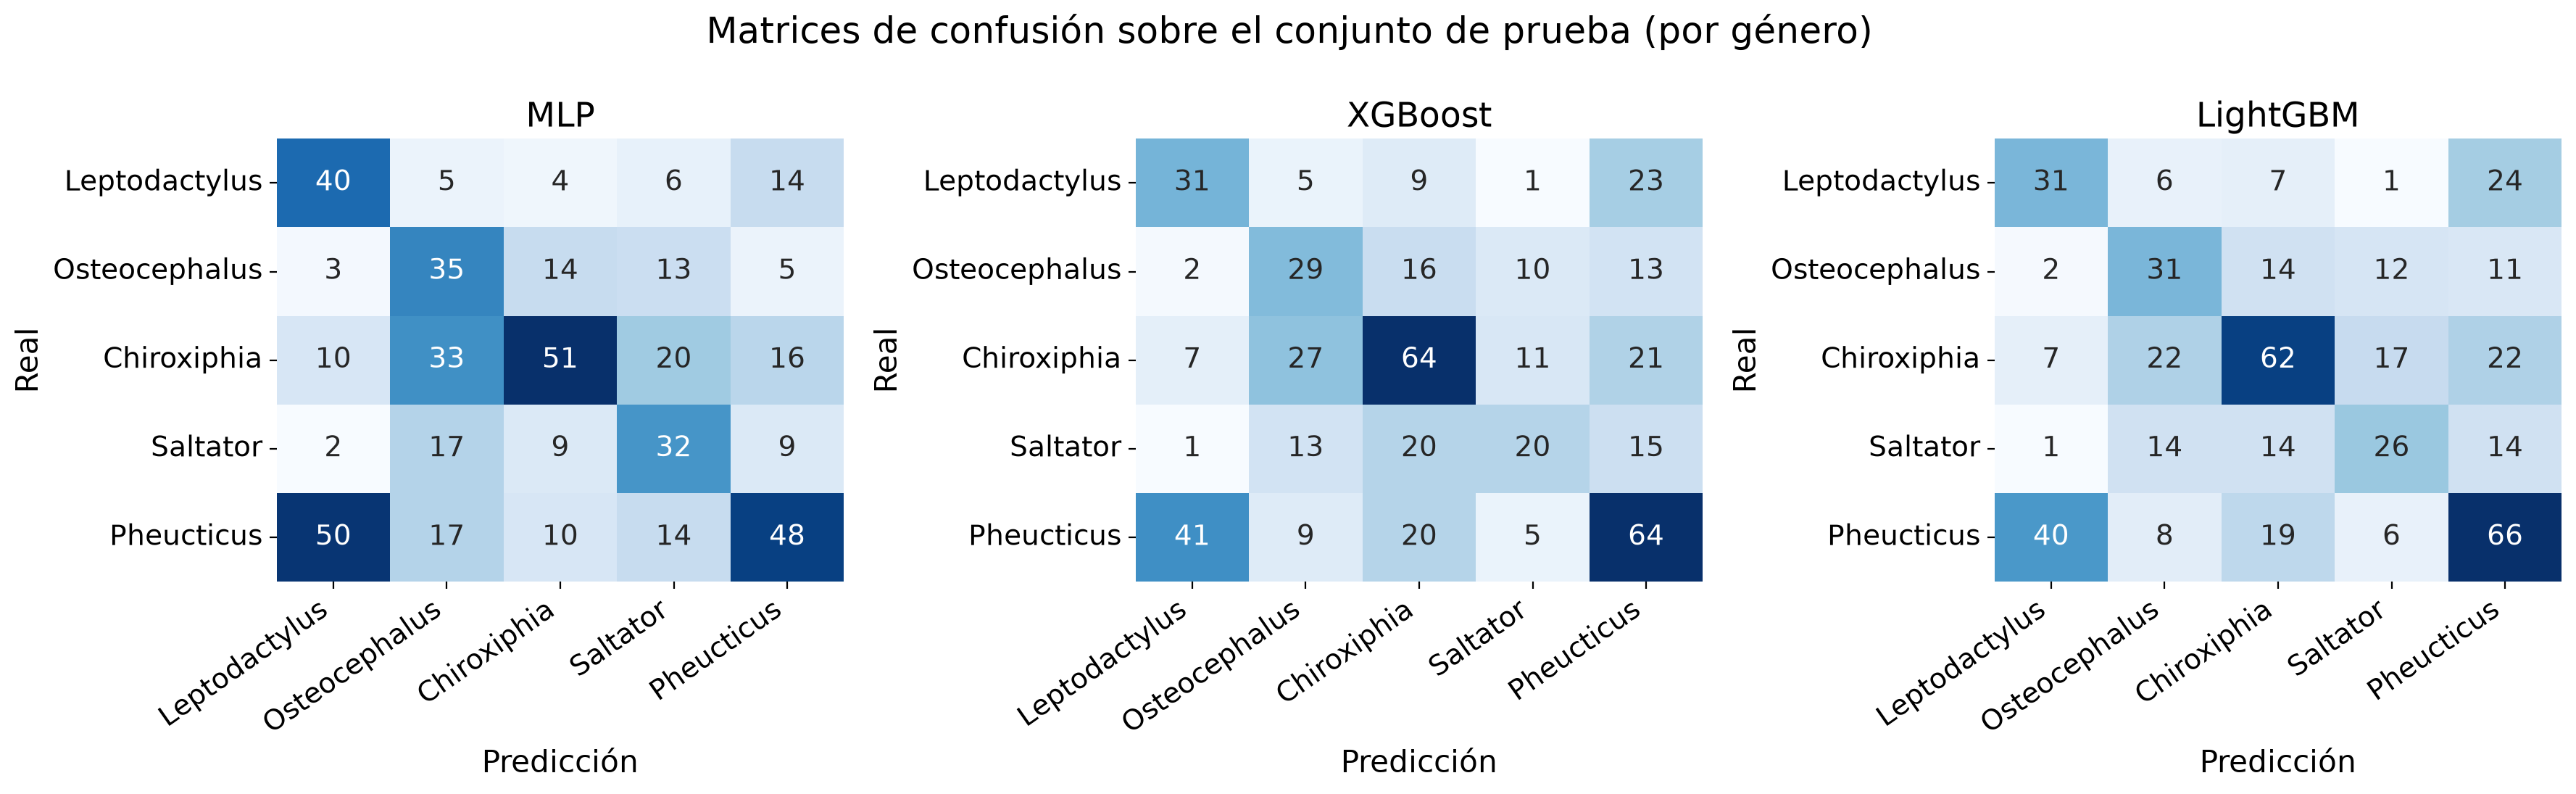
\includegraphics[width=\textwidth]{clf_confusion_matrices.png}
\caption{Matrices de confusión sobre el conjunto de prueba (etiquetadas por género).
Los tres modelos exhiben confusión sistemática, coherente con el solapamiento
geométrico observado.}
\label{fig:cm}
\end{figure*}

\section{Decisiones de Ingeniería y Mitigación de Riesgos}

\textbf{Trade-off costo/rendimiento.} Se midió el tiempo de inferencia mediano por
modelo (Fig.~\ref{fig:inf}): el MLP requiere $\approx$140~ms por cada 1000 muestras
frente a $\approx$3{.}4~ms (XGBoost) y $\approx$4{.}8~ms (LightGBM). Los ensambles
resultan, por tanto, 30--40 veces más rápidos y simultáneamente más precisos, por lo
que LightGBM constituye la elección dominante en la frontera costo--rendimiento para
el despliegue.

\begin{figure}[!t]
\centering
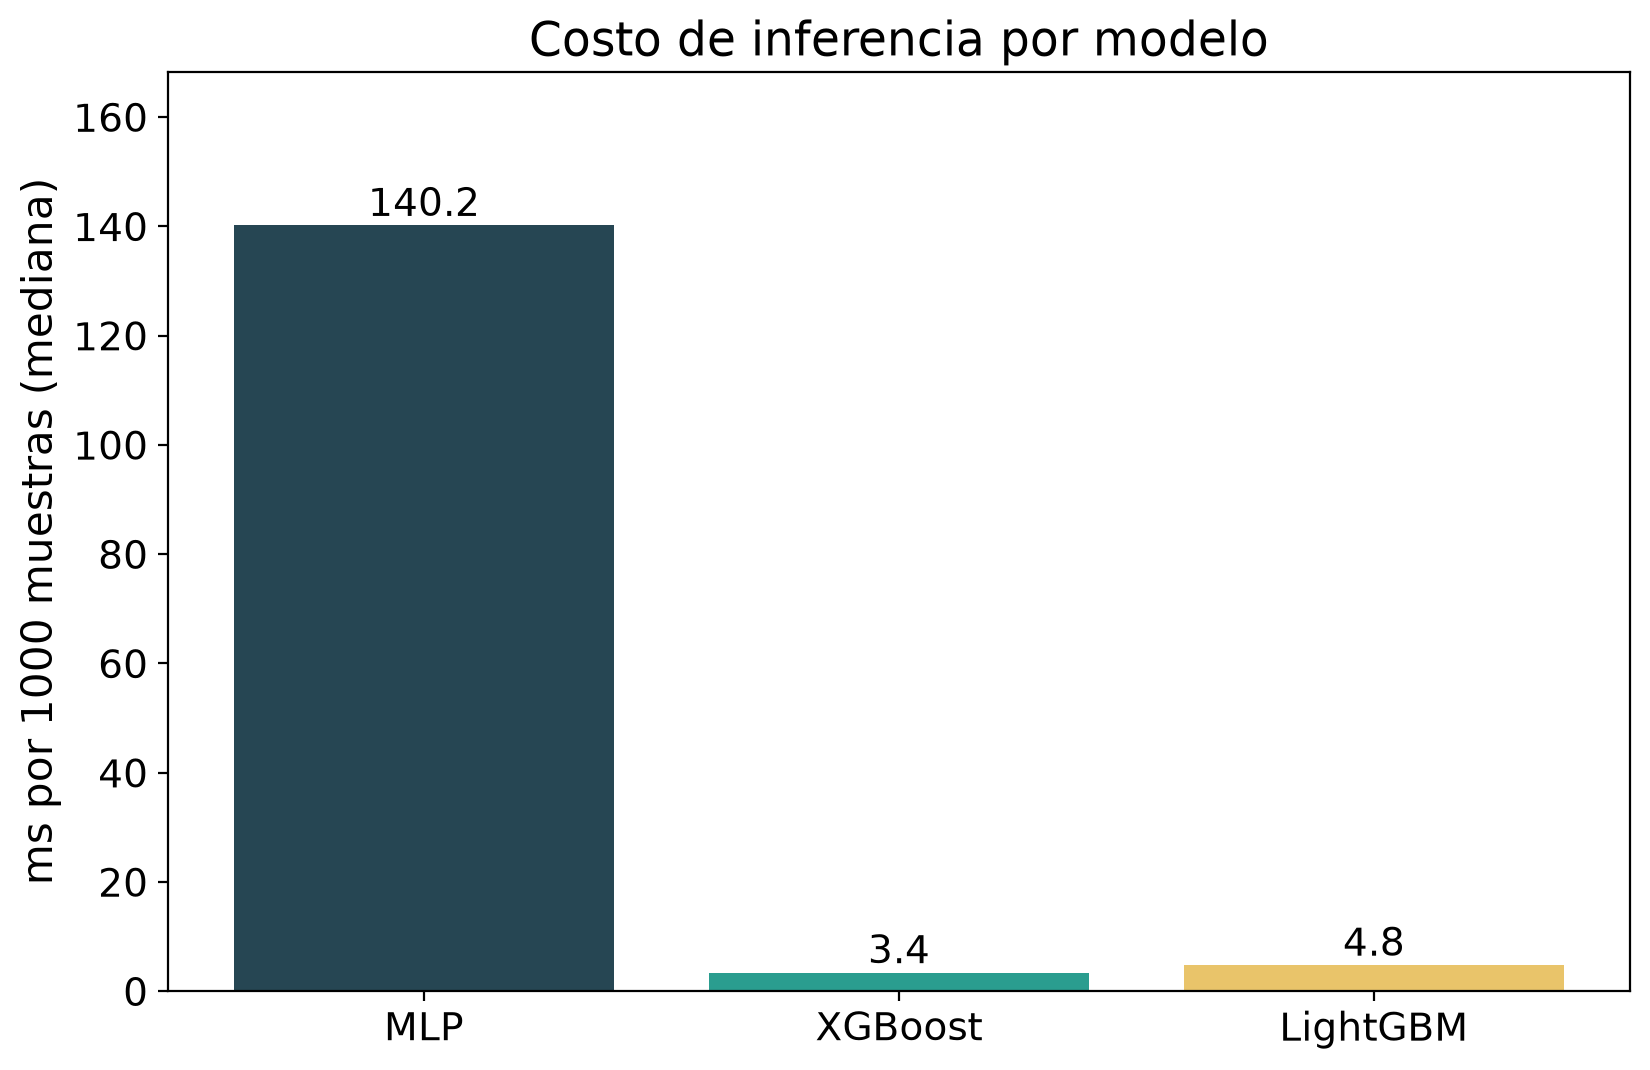
\includegraphics[width=\columnwidth]{thr_inference.png}
\caption{Costo de inferencia mediano por modelo. El MLP es un orden de magnitud más
costoso que los ensambles.}
\label{fig:inf}
\end{figure}

\textbf{Políticas de moderación por umbrales.} Sobre el vector de probabilidad de
LightGBM se definió la confianza $P=\max_k p_k$ y se aplicaron las tres zonas
operativas prescritas (Fig.~\ref{fig:zones}, Tabla~\ref{tab:zones}). El análisis
arrojó un hallazgo de ingeniería relevante: bajo el umbral prescrito del 85\,\%, la
zona de clasificación automática captura apenas el 0{.}2\,\% de las detecciones (1 de
477), pues el solapamiento entre especies impide que el modelo alcance alta
confianza. La mayoría (69\,\%) cae en la zona de auditoría (40--85\,\%) y el 30{.}8\,\%
en rechazo ($<$40\,\%). En consecuencia, se recomienda recalibrar los umbrales a
partir de la curva exactitud--cobertura en lugar de adoptar el 85\,\% nominal, de modo
que la cola de auditoría humana sea operativamente sostenible. Asimismo, la tasa de
\texttt{is\_tp} no aumenta en la zona de mayor confianza, lo que indica que la
confianza del modelo no sustituye la verificación de la etiqueta: el umbral debe
entenderse como mecanismo de control de carga y descarte de ruido, no como garantía de
veracidad biológica.

\begin{table}[!t]
\caption{Zonas de moderación (modelo base: LightGBM).}
\label{tab:zones}
\centering
\begin{tabular}{lccc}
\toprule
Zona & \% & Exactitud & Tasa is\_tp \\
\midrule
Confianza ($\geq$85\,\%)      & 0.2  & ---   & --- \\
Incertidumbre (40--85\,\%)    & 69.0 & 0.474 & 0.128 \\
Rechazo ($<$40\,\%)           & 30.8 & 0.401 & 0.157 \\
\bottomrule
\end{tabular}
\end{table}

\begin{figure}[!t]
\centering
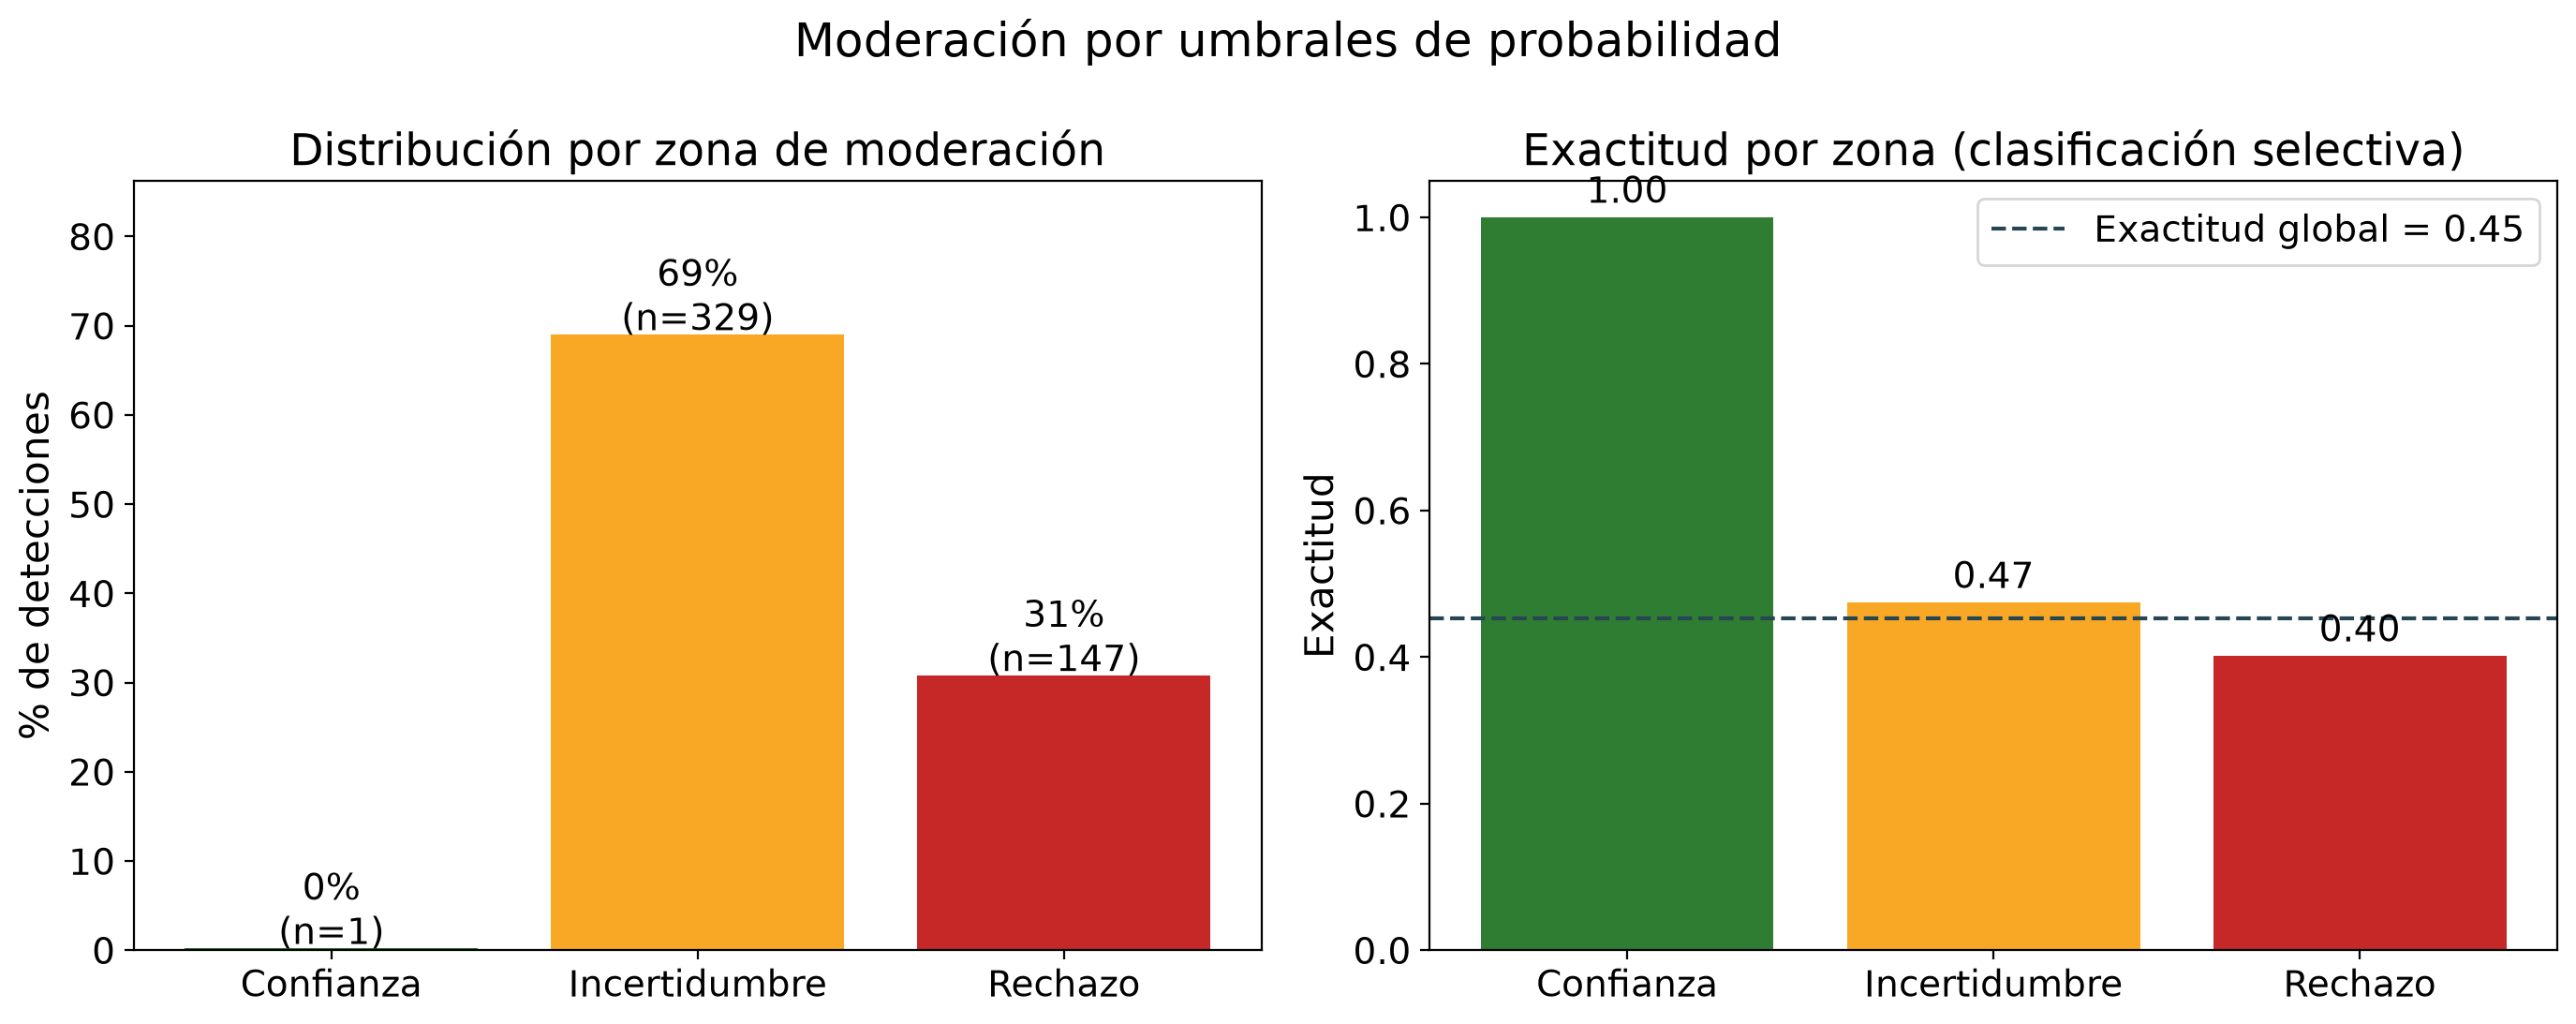
\includegraphics[width=\columnwidth]{thr_zones.png}
\caption{Distribución y exactitud por zona de moderación. La zona de confianza
($\geq$85\,\%) es prácticamente inalcanzable bajo el solapamiento observado.}
\label{fig:zones}
\end{figure}

\section{Conclusiones}

Se desarrolló un pipeline integral de clasificación eco-acústica cuyo principal
hallazgo es el fuerte solapamiento inter-especie en el espacio MFCC: ningún método no
supervisado recupera la etiqueta biológica y los clasificadores supervisados alcanzan
un F1-macro de $\approx$0{.}44, dominado por LightGBM con un costo de inferencia
marcadamente inferior al del MLP. La política de moderación prescrita resultó
inoperante en su umbral nominal, por lo que se propuso su recalibración basada en la
curva exactitud--cobertura. Como trabajo futuro se plantea enriquecer el espacio de
características más allá de los MFCC condensados y modelar explícitamente la
incertidumbre de etiqueta (\texttt{is\_tp}) durante el entrenamiento.

\appendices
\section{Contribution Statement}

\begin{table}[!h]
\caption{Matriz de coevaluación del equipo de desarrollo.}
\label{tab:coeval}
\centering
\begin{tabular}{p{2.4cm}cp{3.2cm}}
\toprule
Integrante & \% Contrib. & Tareas encargadas \\
\midrule
Leonardo Martinez & 100\,\% & [Placeholder: detallar tareas] \\
Marcelo Rosillo & 67\,\% & [Placeholder: detallar tareas] \\
Miguel Paucar & 5\,\% & [Placeholder: detallar tareas] \\
\bottomrule
\end{tabular}
\end{table}

\begin{thebibliography}{9}
\bibitem{umap} L.~McInnes, J.~Healy, and J.~Melville, ``UMAP: Uniform Manifold
Approximation and Projection for Dimension Reduction,'' \emph{arXiv:1802.03426}, 2018.
\bibitem{tsne} L.~van der Maaten and G.~Hinton, ``Visualizing Data using t-SNE,''
\emph{J. Mach. Learn. Res.}, vol.~9, pp.~2579--2605, 2008.
\bibitem{xgboost} T.~Chen and C.~Guestrin, ``XGBoost: A Scalable Tree Boosting
System,'' in \emph{Proc. ACM SIGKDD}, 2016, pp.~785--794.
\bibitem{lightgbm} G.~Ke \emph{et al.}, ``LightGBM: A Highly Efficient Gradient
Boosting Decision Tree,'' in \emph{Proc. NeurIPS}, 2017.
\bibitem{dropout} N.~Srivastava \emph{et al.}, ``Dropout: A Simple Way to Prevent
Neural Networks from Overfitting,'' \emph{J. Mach. Learn. Res.}, vol.~15,
pp.~1929--1958, 2014.
\bibitem{batchnorm} S.~Ioffe and C.~Szegedy, ``Batch Normalization: Accelerating Deep
Network Training by Reducing Internal Covariate Shift,'' in \emph{Proc. ICML}, 2015.
\bibitem{silhouette} P.~J. Rousseeuw, ``Silhouettes: A Graphical Aid to the
Interpretation and Validation of Cluster Analysis,'' \emph{J. Comput. Appl. Math.},
vol.~20, pp.~53--65, 1987.
\end{thebibliography}

\end{document}
